\graphicspath{{fig/missing/}}

\chapter{Missing data}
\label{cha:missing}

Collecting data of flocking events is a demanding process. Along with the
technical challenges posed by data collection, flocking events are inherently
unpredictable, and so it is not possible to know when and where a flocking
event may occur next. In this way there can become a frustrating
`right-place-right-time' component to data collection.

Typically, recording equipment is set up in a fixed location where the
scientist believes an event may occur. Stationary recording equipment results
in a fixed field of vision in which the practitioner may record data.
Unfortunately, this stationary set up can result in recording incomplete
flocking events. This may happen when flock members stray outside the field of
vision during a recording event. The fixed recording equipment means the
field-of-vision cannot be adjusted to reinclude those who move out-of-frame.

The flock members which move out-of-frame cannot simply be ignored during
analysis: although we may not observe their movements, they may still be
influencing the behaviour of the observed flock, and so must be accounted for.
Equally undesirable is the temptation to discard all the frames in which any
individual is out of vision, as this has the potential to drastically reduce
the amount of available data, and to wantonly discard the information it
contains.

In this chapter we will consider how we can handle flocking events which
contain missing observations. Working in a Bayesian framework allows us to
adjust our posterior beliefs about model parameters to account for unobserved
behaviours. We will see that this can be achieved by integrating over all 
possible unobserved paths.

\section{Types of missingness}

When we consider flocking events with missing observations, it is important to
consider at which point during the sequence the data went missing. This is
because how we handle the missingness will depend on at which point during the
sequence the agent went missing.

Although there are many different circumstances which can result in an agent
leaving our field-of-vision, here we shall consider the two cases which we
consider as the most likely to occur. These two cases arise when agents are
out-of-frame at the \emph{beginning} of a recorded flocking event, or when
agents are out-of-frame at the \emph{end} of a recorded event.

We shall integrate over all the possible missing paths within a
Metropolis--Hastings scheme. A proposal mechanism for generating paths missing
at the beginning of a sequence is outlined. Proposed paths can then be accepted
or rejected using results from \cref{cha:sim_studies}. We will then show that
we can generate paths missing at the end of a sequence by performing a Gibbs
step; sampling from our full conditional distributions about the missing
directions of motion.

\subsection{Missing in the beginning}

We say that data is missing at the beginning of a flocking event if the
observer began recording the sequence before all agents had entered the frame.
When we consider this case we assume that all the flock members do eventually
enter the field-of-vision, and so we know the total number of individuals.

\subsection{Missing in the end}

\subsection{Missing in the beginning and end}

\section{Simulation studies}

\subsection{Missing in the beginning}

\begin{figure}[tbp]
  \captionsetup[subfigure]{oneside,
                           margin={0.7cm,0cm}}
  \begin{subfigure}[b]{0.5\textwidth}
    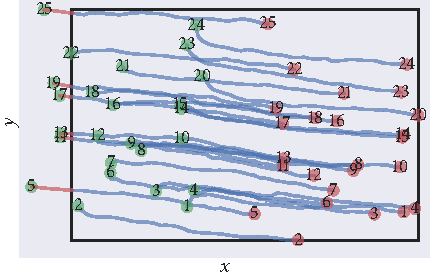
\includegraphics{beg/data.pdf}
    \caption{}
    \label{subfig:beg_data}
  \end{subfigure}%
  \begin{subfigure}[b]{0.5\textwidth}
    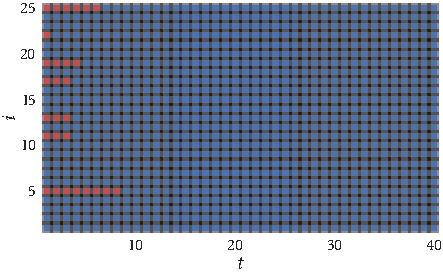
\includegraphics{beg/missing_array.pdf}
    \caption{}
    \label{subfig:beg_missing}
  \end{subfigure}
  \caption{Plots. \subref{subfig:beg_data}
  \subref{subfig:beg_missing}.\lipsum[1]}
\end{figure}

\begin{figure}[tbp]
  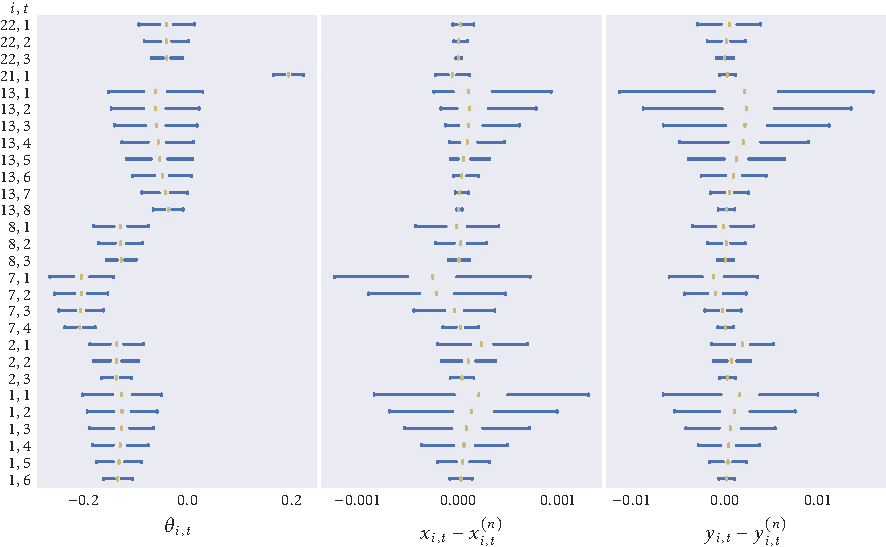
\includegraphics{beg/summary.pdf}
  \caption{caption caption caption}
  \label{fig:beg_summary}
\end{figure}

\begin{figure}[tbp]
  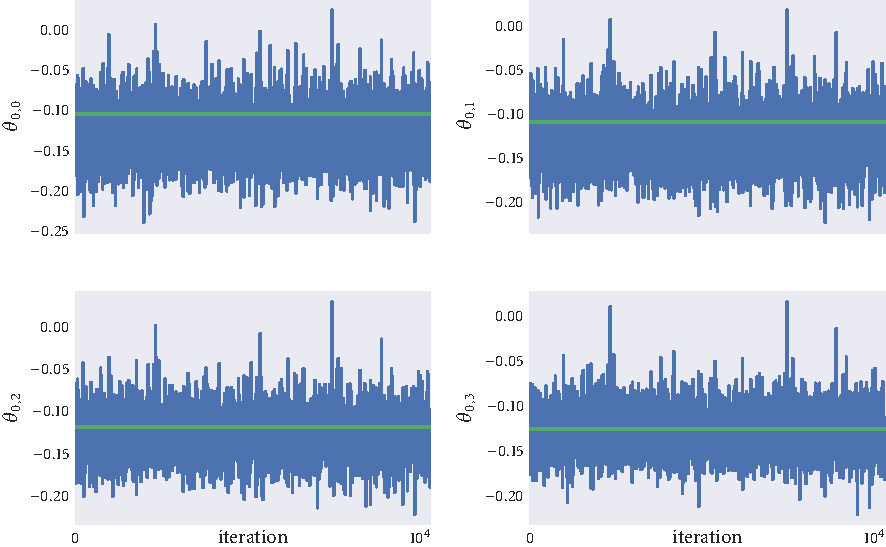
\includegraphics{beg/dir_trace}
  \caption{}
  \label{fig:beg_dir_trace}
\end{figure}

\begin{figure}[tbp]
  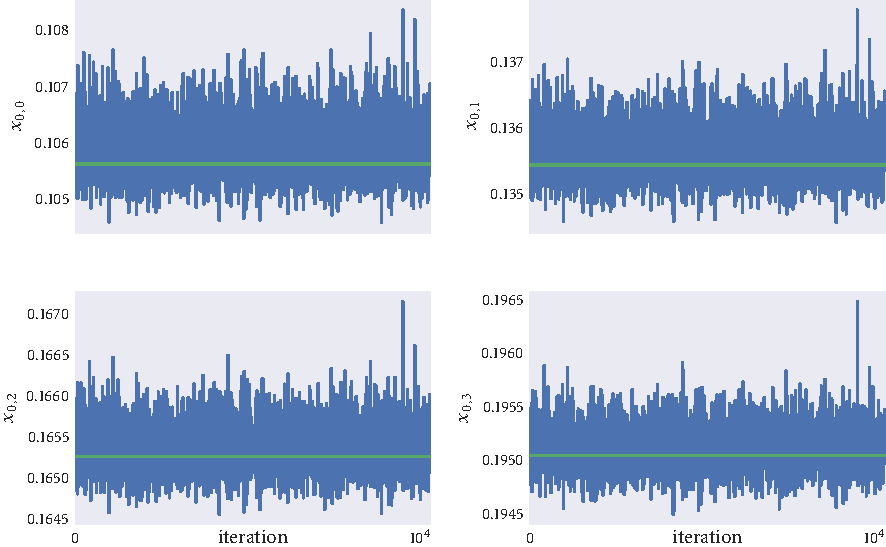
\includegraphics{beg/x_trace}
  \caption{}
  \label{fig:beg_x_trace}
\end{figure}



\subsection{Missing in the end}

\subsection{Missing in the beginning and end}

